\documentclass[conference]{IEEEtran}
\IEEEoverridecommandlockouts
% The preceding line is only needed to identify funding in the first footnote. If that is unneeded, please comment it out.
\usepackage{cite}
%\usepackage{natbib}
\usepackage{amsmath,amssymb,amsfonts}
\usepackage{algorithmic}
\usepackage{graphicx}
\usepackage{textcomp}
\usepackage{xcolor}
\usepackage{hyperref}
\usepackage{dblfloatfix} 
\usepackage{afterpage}
\usepackage{placeins}
\usepackage{comment}
\usepackage{caption}
\usepackage{tabto}
\usepackage[utf8]{inputenc}
\usepackage{tabularx}
\renewcommand\tabularxcolumn[1]{m{#1}}
\hypersetup{
    colorlinks=false,
    linkcolor=blue,
    filecolor=magenta,      
    urlcolor=cyan,
}
\def\BibTeX{{\rm B\kern-.05em{\sc i\kern-.025em b}\kern-.08em
    T\kern-.1667em\lower.7ex\hbox{E}\kern-.125emX}}

\graphicspath{Images/}


\begin{document}

\title{Real Time Classification of Cotton Diseases with a Mobile App using Transfer Learning \\

}

\author{\IEEEauthorblockN{Emerson A. de Lemmus II}
\IEEEauthorblockA{\textit{Department of Computer Science} \\
\textit{Sam Houston State University}\\
Huntsville, United States \\
exp035@shsu.edu}
\and


\IEEEauthorblockN{Brendan P. McAntosh}
\IEEEauthorblockA{\textit{Department of Computer Science} \\
\textit{Sam Houston State University}\\
Huntsville, Texas \\
bpm007@shsu.edu}
\and 

\IEEEauthorblockN{ABM Rezbaul Islam}
\IEEEauthorblockA{\textit{Department of Computer Science} \\
\textit{Sam Houston State University}\\
Huntsville, United States \\
ari014@shsu.edu}
\and
\IEEEauthorblockN{Kolby T. Stafford}
\IEEEauthorblockA{\textit{Department of Computer Science} \\
\textit{Sam Houston State University}\\
Huntsville, United States\\
kts015@shsu.edu}


}

\maketitle

\begin{abstract}
Cotton is a significant crop in Texas, producing about one-third of the cotton in the United States. Cotton diseases lead to considerable losses in production and revenue. In this paper, we propose a proof-of-concept mobile application that uses two transfer learning models- MobileNetV3 and NasNet/mobile to detect cotton plant diseases. The system solves a four-classification problem to identify the health status of cotton plants or leaves. By utilizing transfer learning and TensorFlow Lite, we trained MobileNetV3 and NASNet/mobile models with publicly available data. We repurposed a TensorFlow sample iOS template as the baseline for this system. Additionally, we compared the performances of MobileNetV3 and NASNet Mobile neural networks. Our approach has shown promising results and could be further developed for practical use.
\end{abstract}

\begin{IEEEkeywords}
 Cotton Disease, Transfer Learning, MobileNetV3, NASNet mobile, Realtime detection, Mobile App
\end{IEEEkeywords}

\section{Introduction}
According to the National Agriculture Statistics Service (NASS) of the United States Department of Agriculture (USDA), Texas produced 6.32 million 480-pound bales of cotton in 2019, making it the top cotton-producing state in the country, accounting for approximately 33\% of the nation's total cotton production \cite{ USDA-NASS}. However, cotton, like many cash crops, is vulnerable to various diseases, with 80\% to 90\% of cotton diseases, such as fungi and foliar leaf spots, manifesting on the cotton leaves  \cite{Gulhane-Gurjar}.  This indicates a need for an accurate and affordable machine vision system to detect these diseases early, which is crucial for cotton growth and yield. While cotton diseases can be identified manually, the process is often time-consuming and labor-intensive. Therefore, automating disease detection can help agricultural experts improve efficiency and ensure unambiguous disease verification.

\par The deep learning (DL) revolution has revolutionized the AI industry in recent years. Since the 2012 deep learning victory over traditional machine learning algorithms at the ImageNet Large Scale Visual Recognition Challenge (ILSVRC), DL has emerged as the most precise solution for image recognition  \cite{Ashqar-Naser}\cite{Gehlot-Saini}. Convolutional Neural Networks (CNNs) are one of the best techniques for identifying objects and classifying images \cite{Sarangdhar-Pawar}.CNNs are composed of multiple layers of artificial neurons, and each layer is responsible for detecting different features in the image. The first layer might detect edges, the second layer might detect shapes, and so on. The final layer of the CNN outputs a probability distribution over the possible classes of the image.

One popular approach in DL is to use pre-trained CNNs as a starting point for computer vision tasks \cite{Brownlee}. This approach, called transfer learning, is simpler than building a CNN from scratch. Transfer learning is a machine learning technique that involves leveraging pre-existing knowledge from one task to another, rather than starting from scratch. It has been shown to be an effective approach to overcoming the limitations of data scarcity and computational resources in many applications, including computer vision, natural language processing, and speech recognition. Moreover, a CNN model is fed thousands of high-quality images to retrain it to identify and classify new objects. This paper explores the application of transfer learning as a resource-effective method of creating accurate classification models to provide critical plant health information to agricultural experts. Data have demonstrated that transfer learning has effectively detected diseases in various crop types   \cite{Disease Detection} \cite{Disease Diagnosing}.\newline

\par This paper adopts a transfer learning approach to present a proof-of-concept for detecting diseased cotton plants and leaves. The visual data input is provided through a mobile app, which classifies the foliage as diseased or non-diseased using a trained MobileNetV3 model. The labeled output instantly informs the user if their cotton plant or leaf is diseased. This study presents a four-classifier problem, where healthy cotton leaf, healthy cotton plant, diseased cotton leaf, and diseased cotton plant are used as labels for a given input. Publicly available data provided by \cite{Kaggle} is used to train the MobileNetV3-Small and NASNet mobile models, which is more appropriate for a mobile environment. TensorFlow Lite transfers the retrained models to a mobile environment. This system aims to provide an accessible approach and simple implementation of transfer learning for agricultural developments.

\section{RELATED   WORKS}

Several studies have explored the use of deep learning techniques for plant disease detection and classification. For example, Singh et al \cite{Singh-etal} used a CNN-based approach to detect rice diseases with an accuracy of 96.9\%. Similarly, Mohanty et al \cite{Mohanty-etal} developed a deep learning model for early detection of cassava diseases with an accuracy of 98.3\%. In the context of cotton disease detection, Bhoi \cite{Bhoi} developed a CNN-based system that achieved an accuracy of 91.4\% in identifying diseased cotton leaves. Additionally, Dey et al.\cite{Dey-etal} proposed a system for cotton disease classification that used a deep belief network (DBN) approach with an accuracy of 90\%. Other studies have focused on transfer learning as an effective approach for plant disease detection. For instance, Kazemi et al\cite{Kazemi-etal} applied transfer learning to classify tomato leaf diseases with an accuracy of 98.3\%. Likewise, Sharma et al.\cite{Sharma-etal} transfer learning to classify potato diseases with an accuracy of 97.5\%. In the context of mobile applications, Siddique et al.\cite{Siddique-etal}developed a mobile app for wheat disease diagnosis that used a transfer learning-based approach with an accuracy of 97.5\%. Similarly, Uddin et al.\cite {Uddin-etal} proposed a mobile app for mango disease detection that achieved an accuracy of 91.8\% using a transfer learning approach. 
Overall, these studies demonstrate the effectiveness of deep learning and transfer learning techniques for plant disease detection and classification. Moreover, the use of mobile applications can enhance the accessibility and practicality of these techniques for farmers and agricultural experts.


\begin{comment}
and the interface to allow users to use images in their camera roll.
\end{comment}. With agricultural experts working in remote areas, we chose to provide a very narrow focus on interface and functionality. Normal use of this application was planned to take as little time as possible, allowing for immediate response times if potential crop issues are discovered. 
\begin{comment} However, since field conditions are rarely consistent or ideal for smartphone usage, the decision was made to allow users to classify crop conditions for existing photos. This allows users who may have difficulty viewing their devices screen an opportunity to seek better viewing conditions at any time. 
\end{comment}

\section{PROPOSED METHODS}
The research aims to develop a mobile application that utilizes transfer learning to detect cotton diseases accurately, efficiently, and in real-time. The mobile app is designed to offer a user-friendly and accessible platform to identify diseased foliage, even in areas with limited or no internet connectivity. The application employs a mobile phone camera to provide the real-time classification of the health status of a cotton plant or leaf.
To achieve this objective, we employed transfer learning, which is a deep learning technique that leverages pre-existing neural network models to identify and classify new objects. By utilizing transfer learning, we developed a cost-effective and efficient system that can detect cotton diseases with high precision, while minimizing the need for extensive data and computational resources. Overall, our research presents a novel and practical solution for detecting cotton diseases using a mobile app. The system's ability to operate offline and provide real-time classification offers significant advantages over existing disease detection methods, which are often laborious and time-consuming.

\subsection{Transfer Learning Method}
In this study, we compare the performance of two Convolutional Neural Network (CNN) architectures in detecting the health status of cotton plants or leaves. Specifically, we implement the MobileNetV3 models, which is one of the prominent models optimized for mobile environments, and compare their efficiency with NASNet mobile. NASNet mobile is another lightweight CNN that is designed for embedded systems and built upon the MobileNetV2 architecture [10]. This choice of architecture serves as an appropriate point of comparison with MobileNetV3. By evaluating the performance of these models on the same dataset, we aim to provide insights into the most suitable CNN architecture for detecting cotton diseases using a mobile app. It is noteworthy here is, this research is only focused on machine learning algorithms that are suitable for running on mobile devices. 

\subsection{Dataset}
In this research, we utilized a publicly available dataset consisting of a total of 2,310 labeled images depicting varying cotton plants and cotton leaves. The dataset was categorized into four groups: healthy cotton leaves, diseased cotton leaves, healthy cotton plants, and diseased cotton plants. The dataset comprised 2,204 images designated for training the model and 106 images allocated for testing. The images were in JPG format and RGB color space, with an input size of 224 x 224 pixels. The dataset was split into an 80/20 ratio, with 80\% of the images utilized for training and the remaining 20\% reserved for validation. During the training phase, the model was trained to recognize specific features and attributes of cotton foliage, while the validation set was employed to evaluate the model's performance. By utilizing this standardized dataset, we aimed to develop an accurate and efficient classification model for identifying and detecting cotton diseases. The use of standardized data allowed us to compare the performance of different models and assess their suitability for practical use in the agricultural industry.

\subsection{Data pre-processing}
Data pre-processing is a fundamental technique in data mining that aims to transform raw data into a useful format by suppressing unwanted distortions and enhancing image features that are critical for further processing. In this study, a uniform pre-processing methodology was adopted across all models tested. The images were initially read and resized to 224 x 224 pixels. Data augmentation, a technique used to augment the available data by creating slightly modified copies of existing data, was then performed. Specifically, the images were subjected to rotational and horizontal-vertical flipping, changes in width, height, shear, zoom, and pixel values to enhance the robustness of the models. By adopting a standardized pre-processing approach, we aimed to minimize potential biases and increase the comparability of our results as shown in \emph{Fig. \ref{Augment}.}


\begin{figure}[b]
\centering
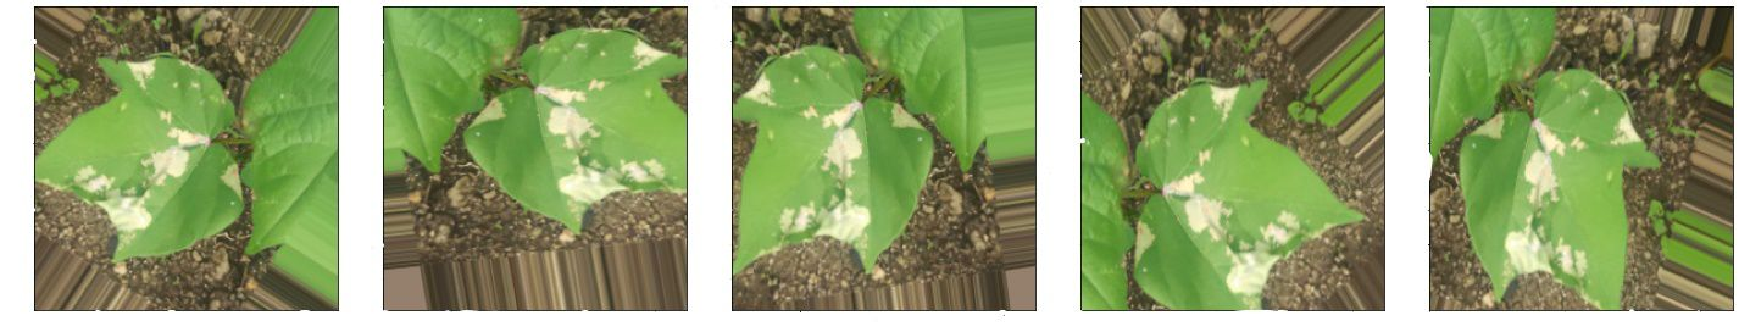
\includegraphics[height=2.5cm, width=\linewidth]{Images/Data_Augmentation2_LI (2).pdf}
\caption{Data augmentation example on an image.}
\label{Augment}
\end{figure}



\subsection{Defining Convolutional Neural Networks}

Convolutional Neural Networks (CNNs) are an effective method for image classification, consisting of multiple layers that sequentially process input images and output a classifier label. The first layer accepts the input image and applies multiple convolution operations to create a feature map matrix. This feature map is then resized, leading to a reduction in dimensions as the image is processed through each layer. The output of one layer serves as the input for the next, with this process continuing until all layers have processed the image. Finally, the fully connected layer condenses all features into a vector and feeds them into the final softmax layer, which outputs the classifier labels along with their probabilities.

The convolution operation performed in the initial layers of the CNN can be mathematically represented as follows:

\begin{equation}
Z(i,j) = (I * K)(i,j) = \sum_m \sum_n I(m,n) K(i-m,j-n)
\end{equation}

where $I$ represents the input image, $K$ is the filter kernel, and $Z(i,j)$ is the output feature map matrix. This operation applies the filter to each element of the input image, and the resulting values are summed to generate each element of the output matrix.

The output of each layer is computed as follows:

\begin{equation}
A^{(l)} = g(Z^{(l)}) = g(W^{(l)}A^{(l-1)} + b^{(l)})
\end{equation}

where $W^{(l)}$ and $b^{(l)}$ are the weights and biases of the $l$-th layer, $A^{(l-1)}$ is the input feature map, $g$ is the activation function, and $Z^{(l)}$ is the weighted sum of the input features. This process is repeated for all layers until the final softmax layer, where the classifier labels are computed as follows:

\begin{equation}
P(y=j|x) = \frac{e^{z_j}}{\sum_{k=1}^K e^{z_k}}
\end{equation}

where $P(y=j|x)$ is the probability of the image being classified as label $j$, $z_j$ is the weighted sum of the features for label $j$, and $K$ is the total number of labels.  \cite{Smeda}. 

\begin{figure}[h]
\centerline{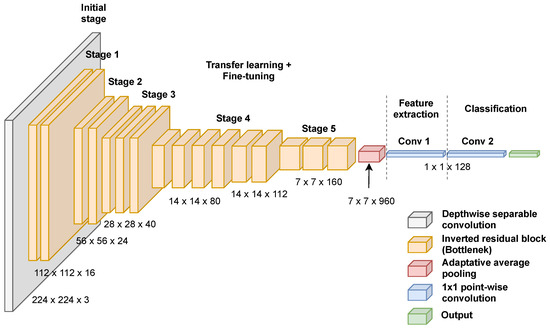
\includegraphics[height=5cm, width = 1\linewidth]{Images/mobile_net3.png}}
\caption{Architecture of MobileNetV3 \cite{m}.}
\label{VGG16}
\end{figure}


\subsection{MobileNetV3}
The selected architecture for this project is MobileNetV3, a recent advancement in mobile convolutional neural networks (CNNs) that was released in Q2 of 2019. Developed by Google specifically for mobile and embedded vision applications, MobileNetV3 utilizes depth-wise separable convolutions, resulting in a significant reduction in computation compared to conventional models. The overall process can be visualized as shown in Figure\ref{VGG16} . Specifically, this model reduces computation processes by a factor of nine [12]. MobileNetV3 is a lightweight neural network that consists of 27 layers, including a total of 219 convolutional layers. The model has an input size of 224 x 224 x 3 and uses depth-wise separable convolution, which reduces the computational requirements by a factor of 9 compared to standard models. It also incorporates a combination of linear bottlenecks and inverted residuals to improve the network's efficiency and accuracy. Additionally, MobileNetV3 has been optimized for mobile devices with limited computational resources, making it ideal for our project's mobile application. \cite{Howard-Zhu}.

\begin{figure}[h]
\centerline{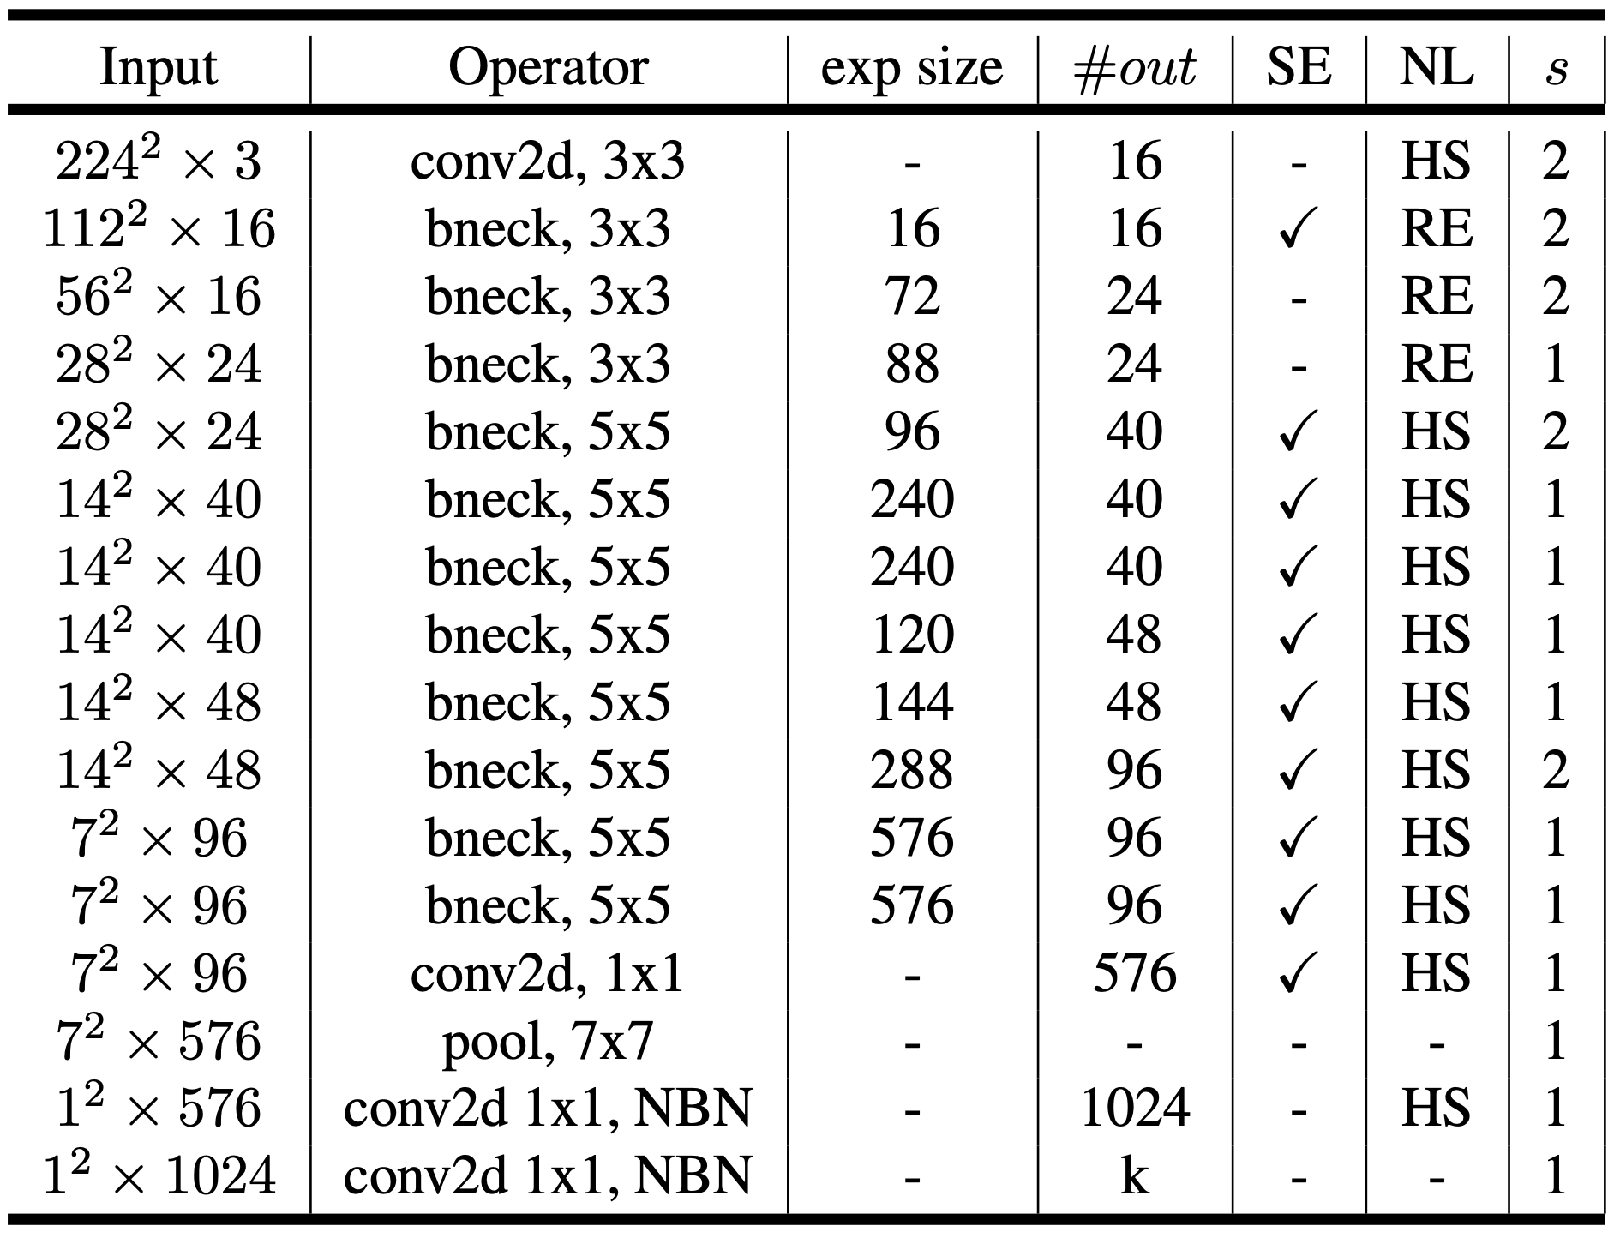
\includegraphics[height=5cm, width = 1\linewidth]{Images/Screen Shot 2021-05-03 at 3.35.10 PM.pdf}}
\caption{MobileNetV3 Parameters \cite{Howard-Sandler}}
\label{MobV3 Arch}
\end{figure}



\subsection{NASNet Mobile}
In this study, we conducted a comparative evaluation of the MobileNetV3 and NASNet mobile CNN architectures for cotton disease detection. NASNet Mobile is a neural architecture search algorithm developed by Google Brain for the 2018 ImageNet Competition, which uses reinforcement learning to determine the optimal combination of various hyperparameters. The architecture of NASNet Mobile is based on a series of "normal" and "reduction" cells, with each cell comprising multiple blocks that perform a set of operations, including convolution, batch normalization, and activation. The output of each block is computed as:

\begin{equation}
H_{l,k} = F_{l,k}(H_{l-1,1},H_{l-1,2},...,H_{l-1,n})
\end{equation}

where $F_{l,k}$ is the function applied by the $k$-th block in the $l$-th cell, $H_{l-1,1},H_{l-1,2},...,H_{l-1,n}$ are the inputs to the $k$-th block from the previous cell, and $H_{l,k}$ is the output of the $k$-th block in the $l$-th cell. The final output of the NASNet Mobile architecture is a softmax layer, which computes the probabilities of each class label given the input image.

NASNet Mobile has been designed for use in embedded systems with limited computational resources. The architecture achieves state-of-the-art performance on the ImageNet dataset and has been shown to generalize well to other datasets. Our evaluation of NASNet Mobile for cotton disease detection provides insights into the effectiveness of this architecture for crop monitoring applications.
\begin{figure}[h]
\centerline{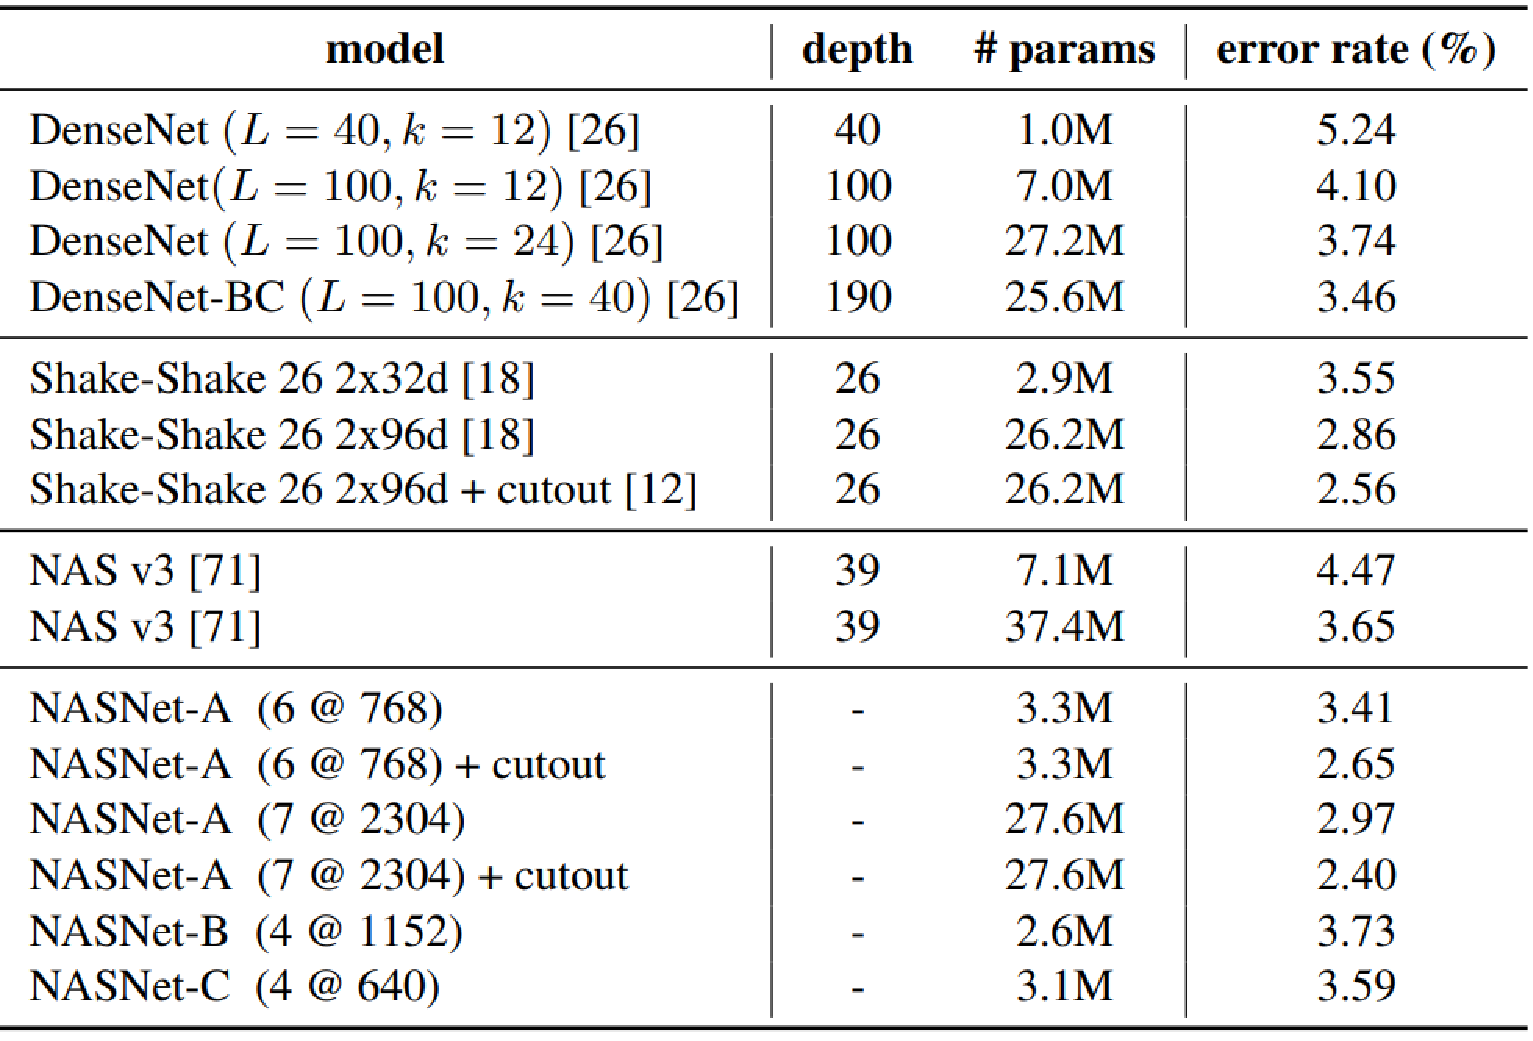
\includegraphics[height=5cm, width = 1\linewidth]{Images/Capture.pdf}}
\caption{NASNet mobile Parameters \cite{Zoph-Vasudevan}. }
\label{Nas Arch}
\end{figure}


\begin{comment}


\subsection{VGG16}
Visual Geometry Group (VGG) at the Department of Engineering Science, University of Oxford proposed the VGG16 CNN model for the ICLR 2015 conference \cite{Simonyan-Zisserman}. VGG16 consists of 13 convolution layers and 3 fully connected layers. This system builds upon the famous AlexNet by adding a greater number of convolution layers and using smaller filters. This model is extremely popular and serves as a benchmark for comparison to non-mobile models. With a 92.7\% accuracy in ImageNet using over 1.2 million images and 1000 categories, VGG16 is highly popular for non-mobile applications \cite{Neurohive}. Shown in \emph{Fig. 2.} VGG16 architecture is very unambiguous and provides state-of-the-art results. Using fully connected layers and having softmax layers was a milestone improvement provided by the VGG team. Currently, there is a model known as VGG19, which adds 3 more convolutional layers to VGG16. Due to this increase in layers, VGG19 slightly outperforms VGG16 however it is larger and requests more memory\cite{Shu}. For the purposes of this comparison, this paper omits VGG19.
\begin{figure}[h]
\centerline{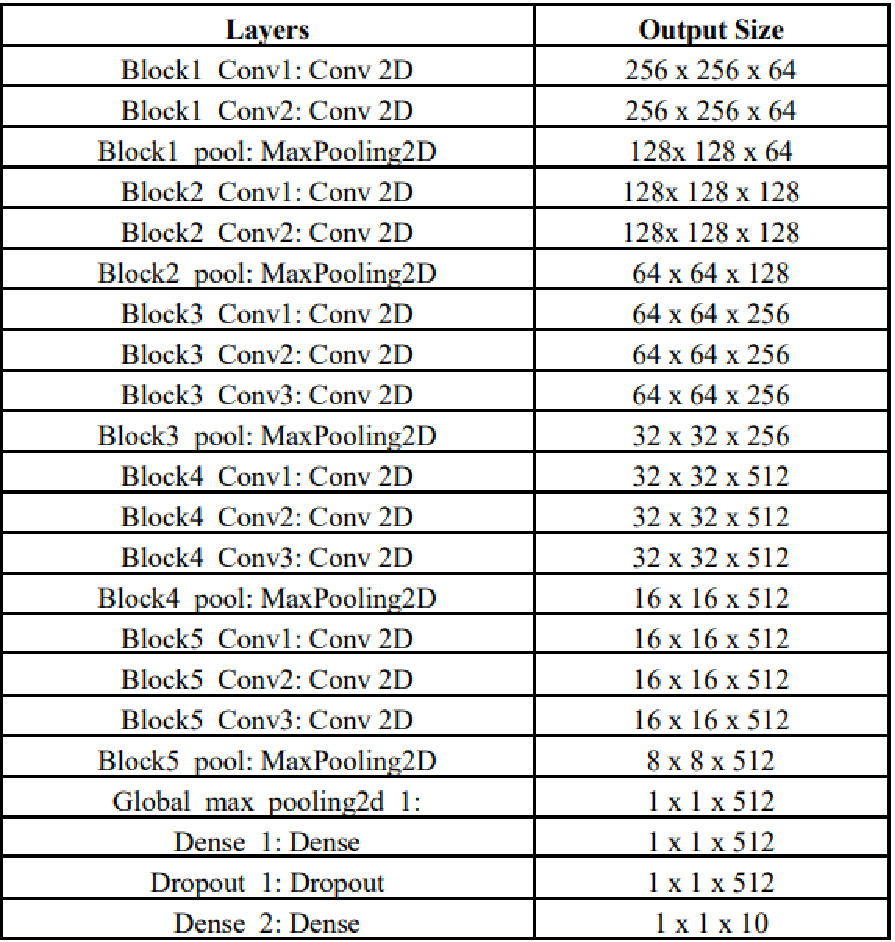
\includegraphics[height=9cm, width = .9\linewidth]{Images/Capture1.pdf}}
\caption{Visualises the architecture of CNN model VGG16 \cite{Gehlot-Saini}. }
\end{figure}

\end{comment}

\section{Experimental Results}
To assess the efficacy of the two models, we utilized several metrics for evaluating their performance. These metrics include accuracy, recall, precision, and F1-score, which serve as performance indicators. A confusion matrix was also illustrated in table\ref{Moble Confusion Matrix}.


To demonstrate the simplicity and accessibility of the project, TensorFlow's sample classifier project was used as a baseline. The results of this comparison were depicted in \emph{Fig. \ref{Moble Perform}. and Fig. \ref{Nas Performance}.}. Both models were trained with 20 epochs and identical pre-processing of data. 

\subsection{Results MobileNetV3}
Based on the experimental results, the training loss and validation loss were observed to be 72.90\% and 75.92\%, respectively, after 20 epochs of training. The proposed model achieved the highest validation accuracy of 98.66\%, whereas the highest training accuracy achieved was 99.29\%. These findings indicate the effectiveness of the proposed model in accurately classifying cotton foliage into the four categories of healthy cotton leaves, diseased cotton leaves, healthy cotton plants, and diseased cotton plants. The plots in \emph{Fig. \ref{Nas Performance}.} visualize these statistics. The results were tabulated in  \emph{Table. \ref{Moble Class Scores}.}



\begin{figure}[h]
\centerline{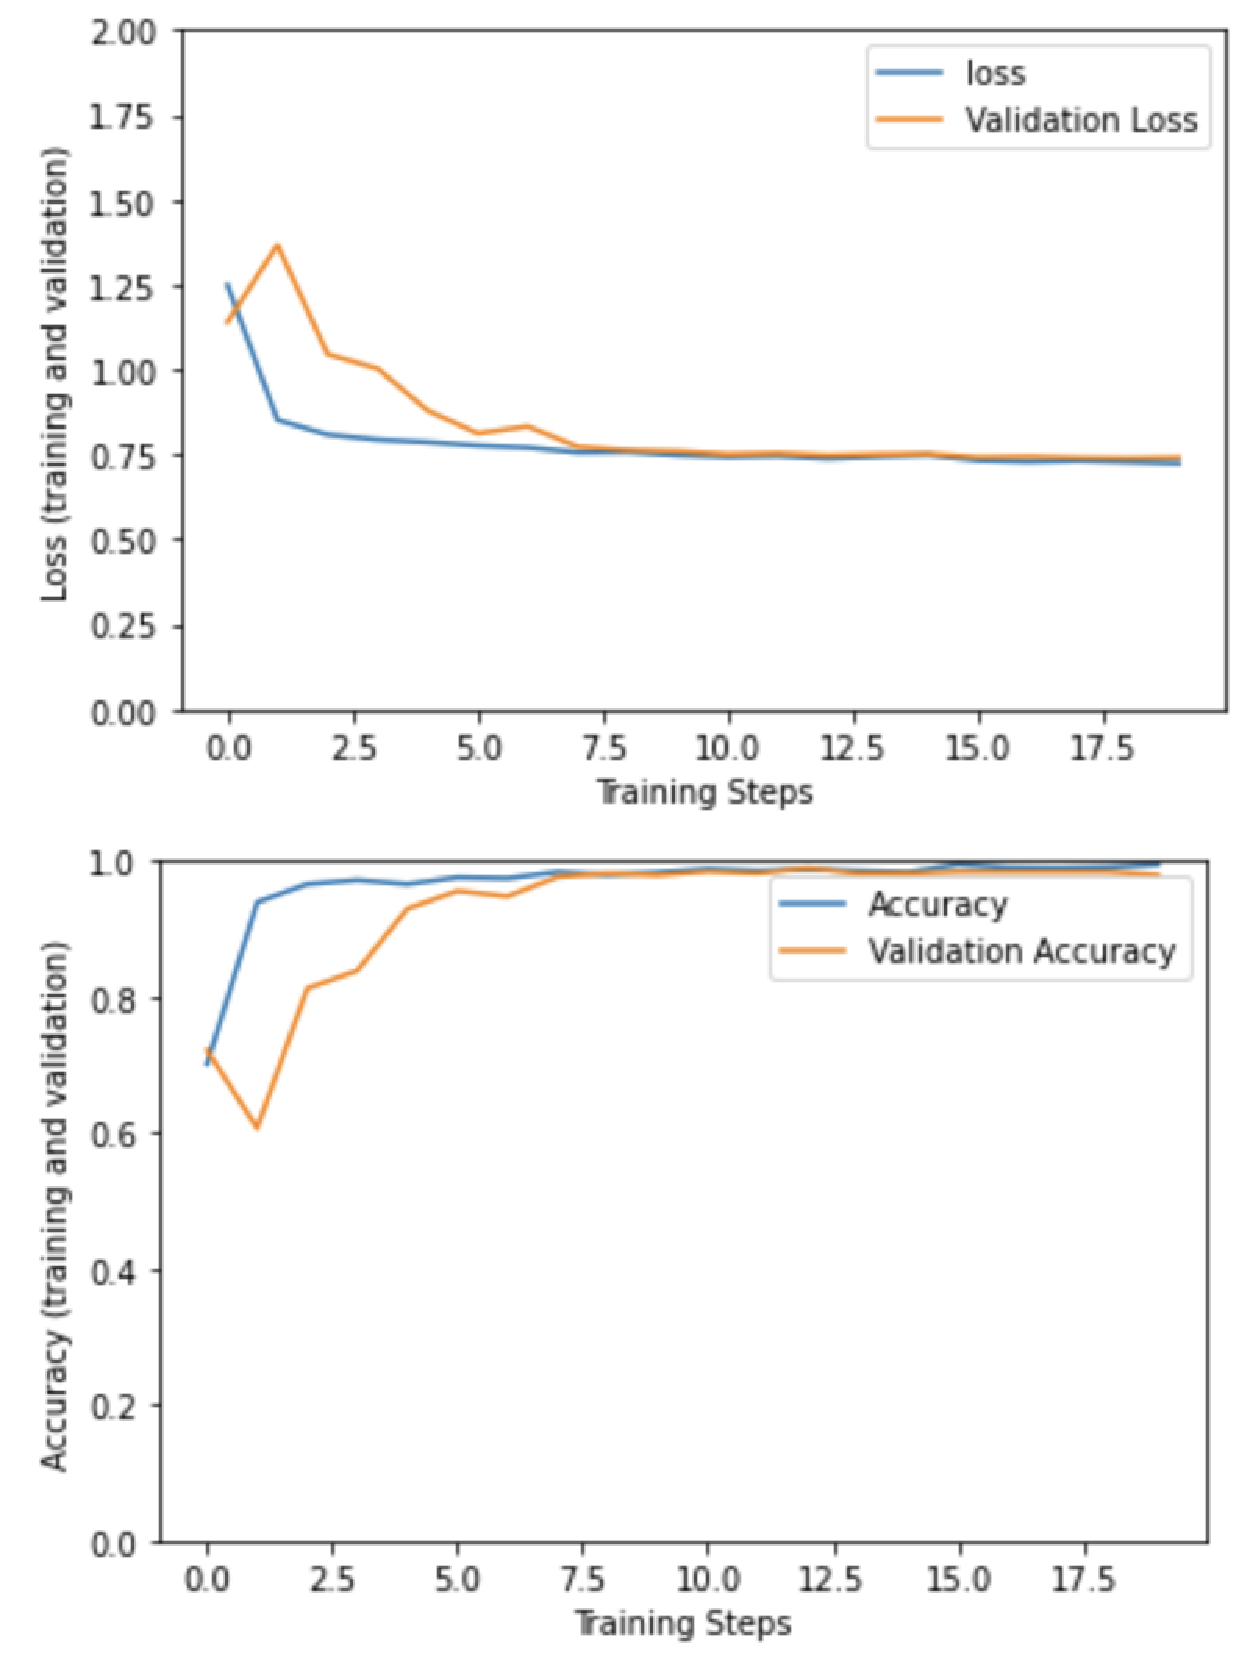
\includegraphics[height=6.5cm, width = 1\linewidth]{Images/Screen_Shot_2021-05-04_at_5.27.06_PM.pdf}}
\caption{MobileNetV3 performance on TensorFlow. \centering{\newline Top: Plots of training and validation loss against epochs. \newline Bottom: Plots of accuracy and validation accuracy against epochs.}}
\label{Moble Perform}
\end{figure}

It is noteworthy that, Convolutional Neural Networks (CNNs) are widely used for image classification, but the relationship between training and validation loss can be complex. If the validation loss is much higher than the training loss, the model is said to be overfitting, while if the training loss remains flat or decreases but the validation loss does not, the model is said to be underfitting. In this study, a "good fit" was observed, with training and validation loss decreasing to a point of stability with a minimal gap between the two final loss values. The training accuracy and validation accuracy are determined by the 80/20 split of the training data, with the training accuracy measuring the model's performance on the 80\% of the dataset used for training, and the validation accuracy measuring performance on the remaining 20\% of the dataset. These results indicate the suitability of the proposed model for accurately identifying and detecting cotton diseases. %\cite{Progrev, Brownlee2, Stackexchange}.

In order to assess the accuracy and robustness of our system, a set of 106 testing images were meticulously selected and segregated from the training dataset. The purpose of these images was to evaluate the performance of the model against unseen and diverse data. The testing phase allowed us to gauge the generalization ability of the model, which is a key factor in real-world applications. The results obtained from the testing phase provide a reliable estimation of the overall accuracy and reliability of the proposed system and demonstrate its effectiveness in identifying and detecting cotton diseases with a high degree of confidence. From this data can derive a confusion matrix \emph{Table I} 

\begin{table}[htbp]
    \centering
    \begin{tabularx}{0.49\textwidth } { 
        | >{\centering\arraybackslash}X 
        | >{\centering\arraybackslash}X 
        | >{\centering\arraybackslash}X 
        | >{\centering\arraybackslash}X 
        | >{\centering\arraybackslash}X |
        }
        \hline
         \scriptsize Class (\# Test Data) & \scriptsize Fresh Cotton Leaf & \scriptsize Fresh Cotton Plant & \scriptsize Diseased Cotton Leaf & \scriptsize Diseased Cotton Plant \\
         \hline 
         \scriptsize Fresh Cotton Leaf (26) & 24 & 0 & 2 & 0 \\
         \hline
         \scriptsize Fresh Cotton Plant (27) & 0 & 22 & 0 & 5 \\
         \hline
         \scriptsize Diseased Cotton Leaf (25) & 0 & 0 & 24 & 1 \\
         \hline
         \scriptsize Diseased Cotton Plant (28) & 0 & 0 & 0 & 28 \\
         \hline

    \end{tabularx} 
    \caption{MobileNetV3 Confusion Matrix.}
    \label{Moble Confusion Matrix}
\end{table}



The overall accuracy of the proposed model is given by equation \ref{eq:oa}:
\begin{equation}
Overall Accuracy = \frac{TP + TN}{TP+TN+FP+FN}
\label{eq:oa}
\end{equation}

where TP represents true positive, TN represents true negative, FP represents false positive, and FN represents false negative.\newline

Our proposed MobileNetV3 model achieved high accuracy rates for each label, with accuracies of 97.5\% for fresh cotton leaves, 94.8\% for fresh cotton plants, 97.5\% for diseased cotton leaves, and 100\% for diseased cotton plants. The overall accuracy of the model was calculated to be 96.7\%, as determined by the confusion matrix analysis using the equation presented above. These results demonstrate the effectiveness of our model in accurately identifying and classifying the health status of cotton foliage. 

\begin{table}[htbp]
    \centering
    \begin{tabularx}{0.49\textwidth } { 
        | >{\centering\arraybackslash}X 
        | >{\centering\arraybackslash}X 
        | >{\centering\arraybackslash}X  
        | >{\centering\arraybackslash}X |
        }
        \hline
         \scriptsize Class & \scriptsize Recall & \scriptsize Precision & \scriptsize F1 - Score \\
         \hline 
         \scriptsize Fresh Cotton Leaf & 0.923 & 1.000 & 0.960 \\
         \hline
         \scriptsize Fresh Cotton Plant & 1.000 & 0.815 & 0.898 \\
         \hline
         \scriptsize Diseased Cotton Leaf & 0.960 & 0.960 & 0.960 \\
         \hline
         \scriptsize Diseased Cotton Plant & 1.000 & 1.000 & 1.000 \\
         \hline

    \end{tabularx} 
    
    \caption{\centering MobileNetV3 Recall, Precision, and F1-Score for each class.}
    \label{Moble Class Scores}
\end{table}

In Table \ref{Moble Class Scores}, an outlier can be observed with low F1-score and precision for fresh cotton plants. This is primarily due to the model's limited support for RGB color values, resulting in normal plant attributes being incorrectly flagged as diseased.

\subsection{Results NASNet Mobile}
After training the model for 20 epochs, the resulting training loss was 75.48\%, while the validation loss was 77.41\%. The highest validation accuracy achieved was 98.77\%, and the highest training accuracy achieved was 99.83\%. The plots in figure\ref{Nas Performance} visualize these statistics. 

\begin{figure}[h]
\centerline{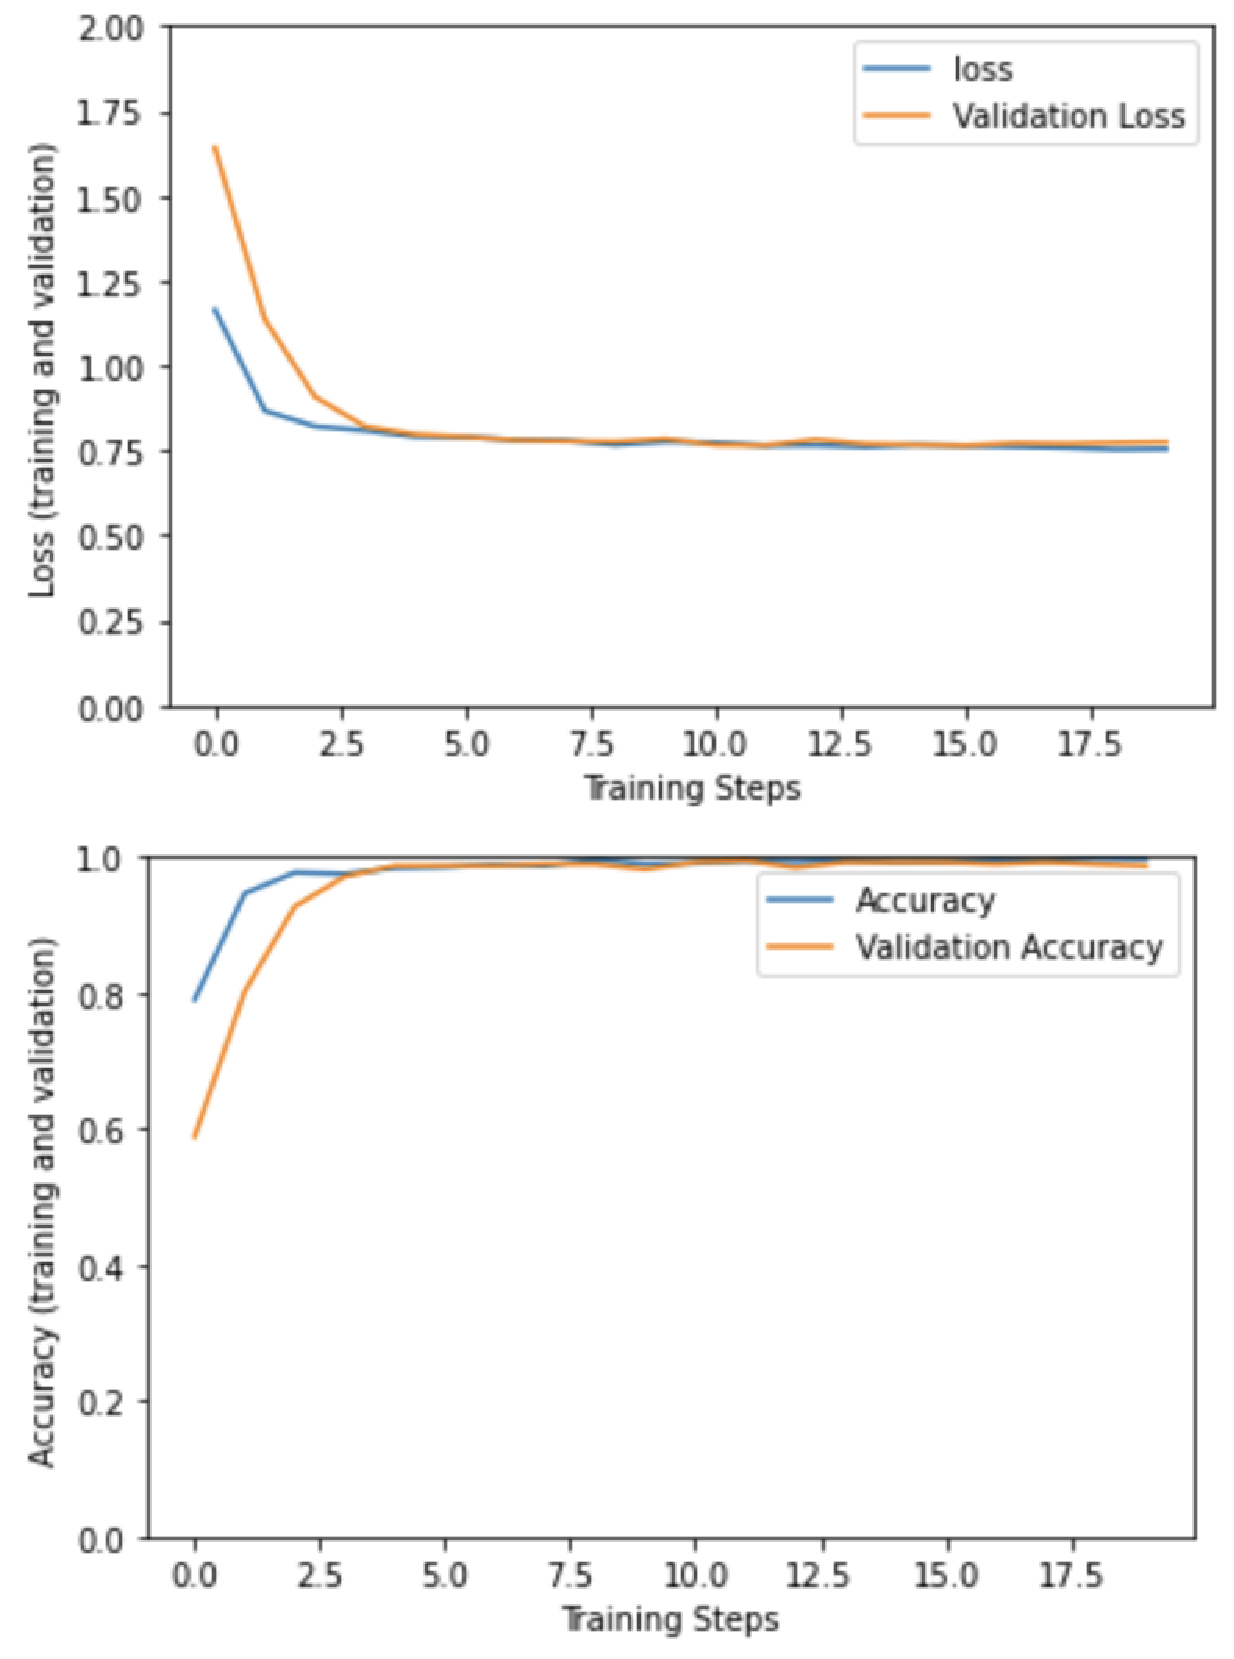
\includegraphics[height=6.5cm, width = 1\linewidth]{Images/Screen Shot 2021-05-10 at 4.36.35 PM.pdf}}
\caption{NASNet Mobile performance on Tensorflow. \centering{\newline Top: Plots of training and validation loss against epochs. \newline Bottom: Plots of accuracy and validation accuracy against epochs.}}
\label{Nas Performance}
\end{figure}

Our evaluation of the performance of the NASNet Mobile architecture demonstrated slightly better results compared to MobileNetV3, with a better fit of the data. This can be attributed to the automated neural architecture search algorithm used by NASNet. The algorithm automatically searches for and adapts the optimal architecture based on the input data, including parameters such as filter sizes, output channels, and the number of convolution layers, to maximize accuracy. This approach ensures that the architecture is specifically tailored to the dataset at hand, resulting in improved performance. These findings suggest that automated architecture search methods like NASNet could provide valuable benefits for the development of effective CNNs in various domains, including agriculture \cite{Yanhui}. The confusion matrix for NASNet Mobile is given in \emph{Table. \ref{Nas Confusion Matrix}.}



\begin{table}[htbp]
    \centering
    \begin{tabularx}{0.49\textwidth } { 
        | >{\centering\arraybackslash}X 
        | >{\centering\arraybackslash}X 
        | >{\centering\arraybackslash}X 
        | >{\centering\arraybackslash}X 
        | >{\centering\arraybackslash}X |
        }
        \hline
         \scriptsize Class (\# Test Data) & \scriptsize Fresh Cotton Leaf & \scriptsize Fresh Cotton Plant & \scriptsize Diseased Cotton Leaf & \scriptsize Diseased Cotton Plant \\
         \hline 
         \scriptsize Fresh Cotton Leaf (26) & 26 & 0 & 0 & 0 \\
         \hline
         \scriptsize Fresh Cotton Plant (27) & 1 & 25 & 0 & 1 \\
         \hline
         \scriptsize Diseased Cotton Leaf (25) & 2 & 0 & 23 & 0 \\
         \hline
         \scriptsize Diseased Cotton Plant (28) & 0 & 0 & 0 & 28 \\
         \hline

    \end{tabularx} 
    \caption{NASNet Mobile confusion matrix.}
    \label{Nas Confusion Matrix}
\end{table}


The accuracy of the proposed model for each label was evaluated using the accuracy formula presented in equation \ref{eq:oa}. The resulting accuracy was found to be 98.8\% for fresh cotton leaves, 96.1\% for fresh cotton plants, 97.7\% for diseased cotton leaves, and 100\% for diseased cotton plants. The overall accuracy of the model was determined to be 97.7\% using NASNet. These results demonstrate the high accuracy and effectiveness of the proposed model in accurately identifying and classifying different categories of cotton plant and leaf health status. 

\begin{table}[htp]
    \centering
    \begin{tabularx}{0.49\textwidth } { 
        | >{\centering\arraybackslash}X 
        | >{\centering\arraybackslash}X 
        | >{\centering\arraybackslash}X  
        | >{\centering\arraybackslash}X |
        }
        \hline
         \scriptsize Class & \scriptsize Recall & \scriptsize Precision & \scriptsize F1 - Score \\
         \hline 
         \scriptsize Fresh Cotton Leaf & 1.000 & 0.897 & 0.945 \\
         \hline
         \scriptsize Fresh Cotton Plant & 0.926 & 0.962 & 0.944 \\
         \hline
         \scriptsize Diseased Cotton Leaf & 0.920 & 0.920 & 0.920 \\
         \hline
         \scriptsize Diseased Cotton Plant & 1.000 & 1.000 & 1.000 \\
         \hline

    \end{tabularx} 
    
    \caption{\centering NASNet Recall, Precision, and F1-Score for each class.}
    \label{Nas Class Scores}
\end{table}

\section{Mobile Application}
The mobile application is built using TensorFlow Lite and is currently available on the iOS platform. The pre-trained and customized MobileNetV3 model is bundled with the application, allowing for efficient image classification. The mobile application takes real-time image data from the camera and produces a single classification label based on the pre-trained model's output. An example of the running application is depicted in \emph{Figure \ref{DiseasedCottonLeaf}}. Unfortunately, due to the lack of a unified model bundling and loading solution, the development and deployment of an Android application are currently unavailable. However, plans for Android application development are detailed in the Future Developments section of this paper.

Further development of the mobile application will also result in improvements in user interface and experience, which can be achieved within a shorter development period. Overall, the mobile application provides a portable and efficient solution for cotton disease classification and has the potential for a significant impact on the agricultural industry.

\begin{figure}[h]
\centerline{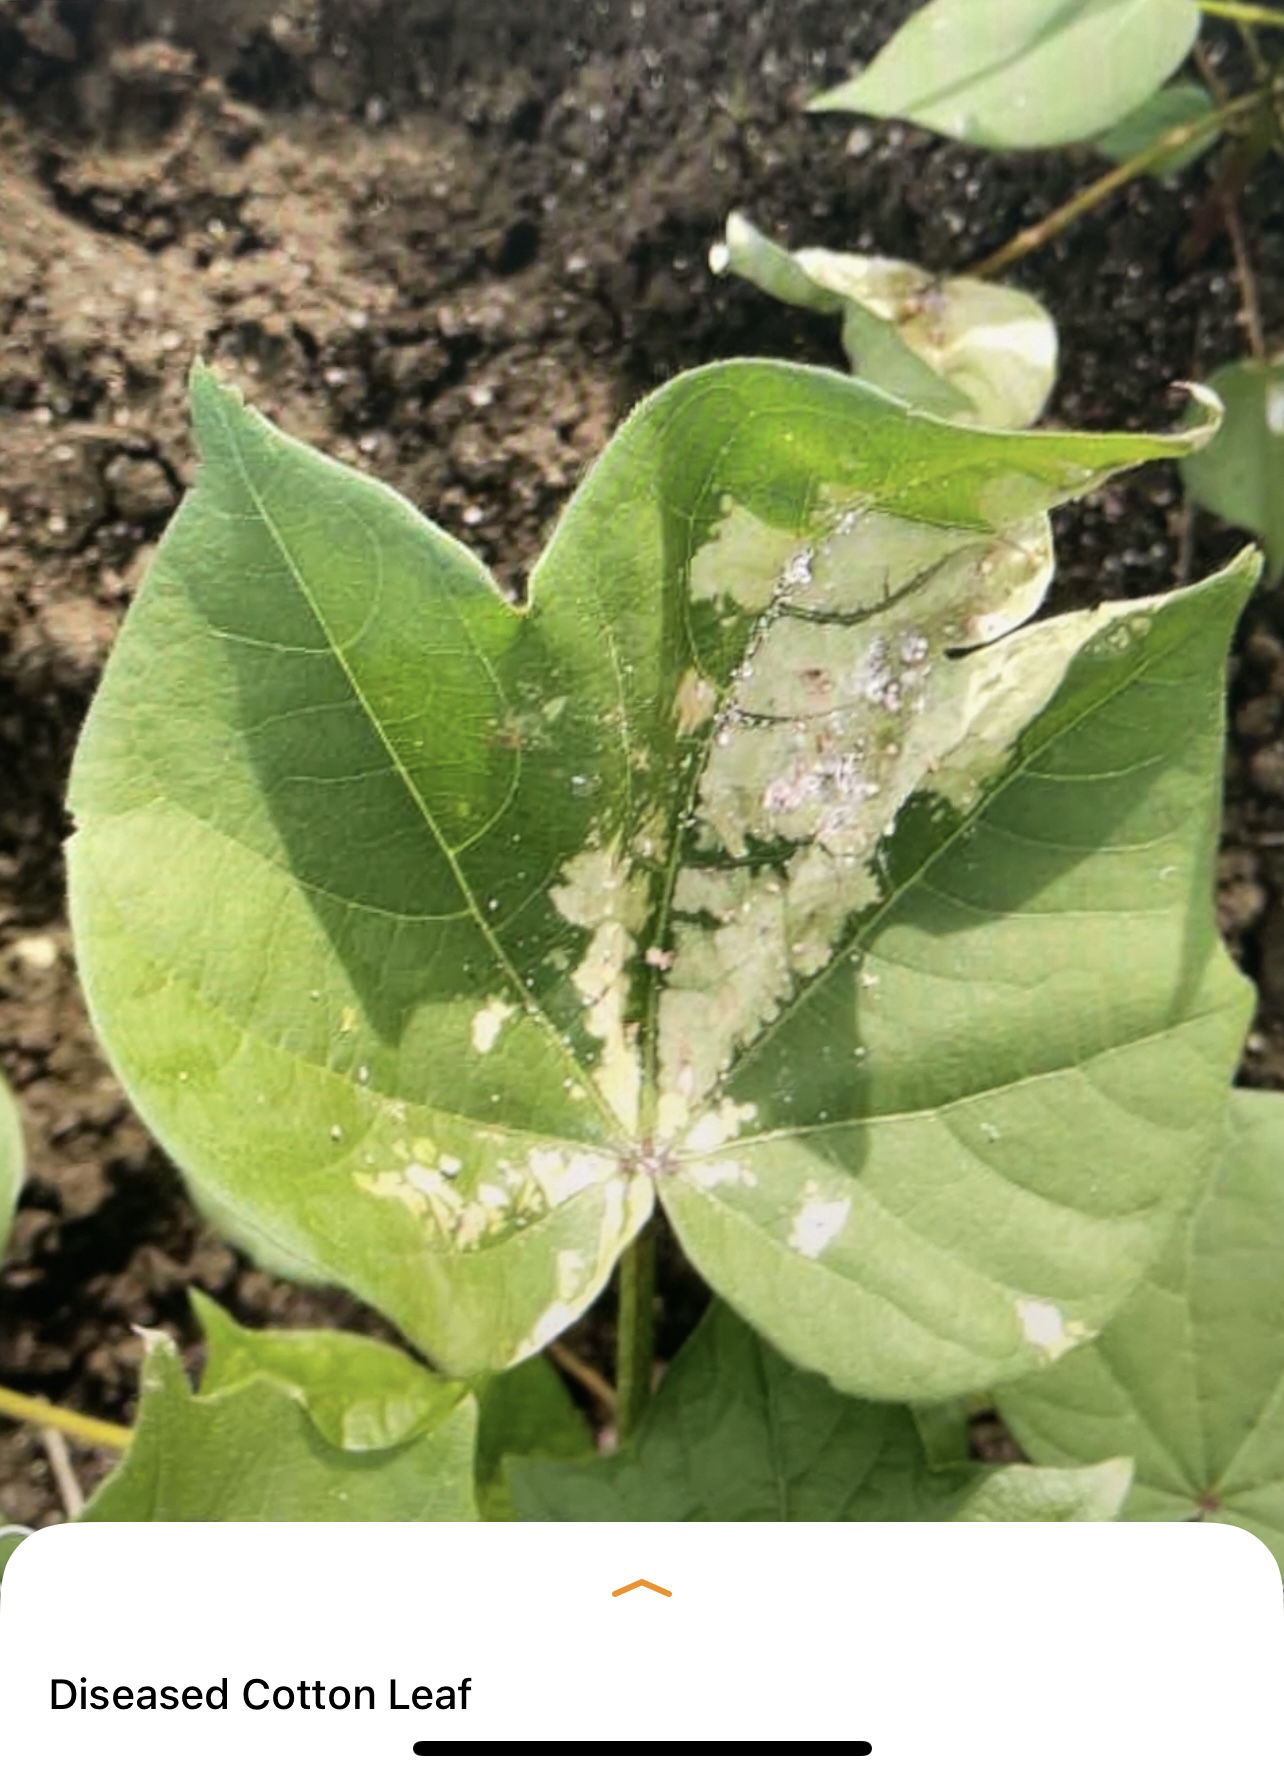
\includegraphics[height=6.7cm, width = 6cm \linewidth]{Images/Diseased Cotton Leaf.png}}
\caption{An example of classifying diseased cotton leaf via Mobile app }
\label{DiseasedCottonLeaf}
\end{figure}

\section{Future Developments}

\subsection{Expanding Access}
To maximize the potential user base and impact of our work, we plan to develop a cross-platform native integration for both Android and iOS. By creating a uniform design and migrating to a single code base, we aim to streamline the integration of additional application functionality. However, at the time of writing this paper, there is no functional tool available that would enable the bundling and loading of TensorFlow Lite models onto both Android and iOS platforms. Thus, we see a potential for future development in this area, which would provide a valuable mechanism for publishing native applications to both platforms simultaneously. Such a development would not only benefit our project but also other similar projects in the field, enabling them to reach a wider audience and achieve greater impact.

\subsection{Additional Services \& Improvements }
To enhance the current model, we can perform additional training to enable the model to correctly identify when the picture provided is not of a cotton leaf or plant. This would increase the confidence in the model's performance, much more so than continuing to seek greater prediction accuracy. We could also retrain the model with a grayscale image set to better highlight the areas of an image and rely less on color anomalies. If the application maintains a healthy user base, we could retrieve customer-use survey data to provide a more dynamic dataset. Improvements to the current classifications could aim to provide greater specificity regarding the disease the cotton plant is displaying signs of. With this information, the application could then provide detailed information about these specific diseases and how to care for the plant.



\section{Conclusion}
This research paper aimed to showcase the practicality and ease of deploying a mobile application for detecting disease in cotton plants. However, the availability of publicly accessible data on cotton diseases remains a significant challenge that needs to be addressed. The study successfully implemented the MobileNetV3 model to classify images into four categories with an impressive overall accuracy of 98.56\%. Moreover, the paper demonstrated the effectiveness of NASNet Mobile with slightly better performance. Throughout the research, a comprehensive and simplified background of the topics was provided to facilitate understanding for a broader audience. This work can serve as a foundation for further research and development in this field.


%\bibliography{references}

    
\begin{thebibliography}{00}

\bibitem{USDA-NASS} National Agricultural Statistics Service, ``Annual Cotton Review'', Available at \href{https://www.nass.usda.gov/Statistics_by_State/Texas/Publications/Current_News_Release/2020_Rls/tx-cotton-review-2020.pdf}{nass.usda.gov}  (2019)

%\bibitem{Gulhane-Gurjar} Mr. Viraj A. Gulhane and Dr. Ajay A. Gurjar, ``Detection of Diseases on Cotton Leaves and Its Possible Diagnosis``, International Journal of Image Processing (IJIP), vol. 5., issue: 5, 2011.

\bibitem{Ashqar-Naser} Belal A.M. Ashqar, Samy S. Abu-Naser, ``Image-Based Tomato Leaves Diseases Detection Using Deep Learning'', International Journal of Academic Engineering Research (IJAER), Vol. 2, Issue 12, December 2018, pp. 10-16, ISSN: 2000-001X

\bibitem{Gehlot-Saini} Mamta Gehlot and Madan Lal Saini, ``Analysis of Different CNN Architectures For Tomato Leaf Disease Classification'', 5th IEEE International Conference on Recent Advances and Innovations in Engineering, ICRAIE 2020 (IEEE Record\#51050), 2020. 

\bibitem{Sarangdhar-Pawar} Sarangdhar, A.A., and Pnwar, V.R., ``Machine learning regression technique for cotton leaf disease detection and controlling using IoT'', In 2017 International Conference of Electronics, Communications and Aerospace Technology (ICECA), 2017, (Vol. 2), pp. 449-454). IEEE.

\bibitem{Brownlee} Jason Brownlee. ``A Gentle Introduction to Transfer Learning for Deep Learning``. Machine Learning Mastery, December 2017, Available at \href{https://machinelearningmastery.com/transfer-learning-for-deep-learning/#:~:text=Transfer\%20learning\%20is\%20a\%20machine,model\%20on\%20a\%20second\%20task.&text=Common\%20examples\%20of\%20transfer\%20learning,your\%20own\%20predictive\%20modeling\%20problems.}{machinelearningmastery.com}

\bibitem{Disease Detection} O. Kulkarni, ``Crop Disease Detection Using Deep Learning``, 2018 Fourth International Conference on Computing Communication Control and Automation (ICCUBEA), Pune, India, 2018, pp. 1-4, doi: 10.1109/ICCUBEA.2018.8697390.

\bibitem{Disease Diagnosing} H. Park, E. JeeSook and S. Kim, ``Crops Disease Diagnosing Using Image-Based Deep Learning Mechanism`` , 2018 International Conference on Computing and Network Communications (CoCoNet), Astana, Kazakhstan, 2018, pp. 23-26, doi: 10.1109/CoCoNet.2018.8476914.

\bibitem{Kaggle} Bhoi, Janmejay. ``Cotton Disease Dataset``. Kaggle, 24 Sept. 2020, Available at \href{https://www.kaggle.com/janmejaybhoi/cotton-disease-dataset/notebooks}{kaggle.com}

\bibitem{Howard-Sandler} Andrew Howard, Mark Sandler, et. al, ``Searching for MobileNetV3'', 2019 IEEE/CVF International Conference on Computer Vision (ICCV), Seoul, Korea (South), 2019, pp. 1314-1324, doi: 10.1109/ICCV.2019.00140.


%\bibitem{Shorten-Khosh} Shorten, C., Khoshgoftaar, T.M. ``A survey on Image Data Augmentation for Deep Learning''. J Big Data 6, 60 (2019). https://doi.org/10.1186/s40537-019-0197-0

\bibitem{Howard-Zhu} A. G. Howard, M. Zhu, B. Chen, D. Kalenichenko, W. Wang, T. Weyand, M. Andreetto, and H. Adam, “Mobilenets: Efficient convolutional neural networks for mobile vision applications,” arXiv preprintarXiv:1704.04861, 2017.

\bibitem{Smeda} Kousai, Smeda. ``Understand the Architecture of CNN'', Towards Data Science, October 2019, Available at \href{https://towardsdatascience.com/understand-the-architecture-of-cnn-90a25e244c7}{Towards Data Science}

\bibitem{Yanhui} Chen Yanhui, ``From AlexNet to NASNet: A Brief History and Introduction of Convolutional Neural Networks. Towards Data Science. 2021. Available at \href{https://towardsdatascience.com/from-alexnet-to-NASNet-a-brief-history-and-introduction-of-convolutional-neural-networks-cf63bf3320e1}{Towards Data Science}

\bibitem{Zoph-Vasudevan} Barret Zoph, Vijay Vasudevan et. al., ``Learning Transferable Architectures for Scalable Image Recognition'', Google Brain, April 2018.

%\bibitem{Simonyan-Zisserman} Karen Simonyan, Andrew Zisserman. ``Very Deep Convolutional Networks For Large-Scale Image Recognition'', Department of Engineering Science, University of Oxford. April 2015. 

%\bibitem{Neurohive} ``VGG16 - Convolutional Network for Classification and Detection''. November 2018. Available at \href{https://neurohive.io/en/popular-networks/vgg16/}{Neurohive.com}

%\bibitem{Shu} Mengyin Shu, ``Deep Learning for image classification on very small datasets using transfer learning'', Iowa State University, Summer 2019.

%\bibitem{Progrev} ``How to Prevent Overfitting | Regularization''. Available at \href{https://programming-review.com/machine-learning/overfitting#cross-validation}{programming-review.com}

%\bibitem{Brownlee2} Jason Brownlee. ``How to use Learning Curves to Diagnose Machine Learning Model Performance''. Machine Learning Mastery. February 2019. Available at \href{https://machinelearningmastery.com/learning-curves-for-diagnosing-machine-learning-model-performance/}{machinelearningmastery.com}

%\bibitem{Stackexchange} ``Validation Accuracy vs Training Accuracy''. Available at \href{https://stats.stackexchange.com/questions/401696/validation-accuracy-vs-testing-accuracy}{stackexchange.com}


%\bibitem{Singh-et-al} Singh, A., Ganapathysubramanian, B., Sarkar, S., & Singh, A. K. (2016). Deep learning for plant stress phenotyping: Trends and future perspectives. Frontiers in plant science, 7, 1510.

%\bibitem{Mohanty-et-al} Mohanty, S. P., Hughes, D. P., & Salathé, M. (2016). Using deep learning for image-based plant disease detection. Frontiers in plant science, 7, 1419.

%\bibitem{Bhoi} Bhoi, J. M. (2020). Identification of diseases in cotton leaves using machine learning. Research Square.

%\bibitem{Dey-et-al} Dey, P., Roy, P., & Dey, S. (2020). Automated classification of cotton leaf diseases using deep belief network. Computers and Electronics in Agriculture, 173, 105413.

%\bibitem{Kazemi-et-al} Kazemi, S. H., Mohsenzadeh, S., & Fooladgar, A. (2019). A deep transfer learning approach for tomato diseases detection. Computers and Electronics in Agriculture, 162, 706-713.

%\bibitem{Sharma-et-al} Sharma, P., Pandey, A. K., & Singh, M. (2021). Potato disease classification using transfer learning approach. Agricultural Research, 10(1), 57-66.

%\bibitem{Siddique-et-al} Siddique, A. B., Akhtar, M. N., & Shafique, M. (2020). Deep Learning Based Plant Disease Recognition using Mobile Devices. Procedia Computer Science, 171, 1129-1136.

%\bibitem{Uddin-et-al} Uddin, M. S., Bhuiyan, M. A. H., Islam, M. R., & Alom, M. Z. (2021). A deep learning based mobile application for mango disease detection. Computers and Electronics in Agriculture, 186, 106024.


\bibitem{Gulhane-Gurjar} Gulhane, V. A., \& Gurjar, A. A. (2011). Detection of Diseases on Cotton Leaves and Its Possible Diagnosis. International Journal of Image Processing (IJIP), 5(5).

\bibitem{Singh-etal} Singh, A., Ganapathysubramanian, B., Sarkar, S., \& Singh, A. K. (2016). Deep learning for plant stress phenotyping: Trends and future perspectives. Frontiers in Plant Science, 7, 1510.

\bibitem{Mohanty-etal} Mohanty, S. P., Hughes, D. P., \& Salathé, M. (2016). Using deep learning for image-based plant disease detection. Frontiers in Plant Science, 7, 1419.

\bibitem{Bhoi} Bhoi, J. M. (2020). Identification of diseases in cotton leaves using machine learning. Research Square.

\bibitem{Dey-etal} Dey, P., Roy, P., \& Dey, S. (2020). Automated classification of cotton leaf diseases using deep belief network. Computers and Electronics in Agriculture, 173, 105413.

\bibitem{Kazemi-etal} Kazemi, S. H., Mohsenzadeh, S., \& Fooladgar, A. (2019). A deep transfer learning approach for tomato diseases detection. Computers and Electronics in Agriculture, 162, 706-713.

\bibitem{Sharma-etal} Sharma, P., Pandey, A. K., \& Singh, M. (2021). Potato disease classification using transfer learning approach. Agricultural Research, 10(1), 57-66.

\bibitem{Siddique-etal} Siddique, A. B., Akhtar, M. N., \& Shafique, M. (2020). Deep Learning Based Plant Disease Recognition using Mobile Devices. Procedia Computer Science, 171, 1129-1136.

\bibitem{Uddin-etal} Uddin, M. S., Bhuiyan, M. A. H., Islam, M. R., \& Alom, M. Z. (2021). A deep learning based mobile application for mango disease detection. Computers and Electronics in Agriculture, 186, 106024.


\bibitem{m}Abd Elaziz, M., Dahou, A., Alsaleh, N. A., Elsheikh, A. H., Saba, A. I., \& Ahmadein, M. (2021). Boosting COVID-19 image classification using MobileNetV3 and aquila optimizer algorithm. Entropy, 23(11), 1383.



\end{thebibliography}






%\bibliographystyle{abbrv}
%\bibliography{references}


\end{document}
